\documentclass{ifacconf}

\usepackage{natbib}            % you should have natbib.sty
\usepackage[utf8]{inputenc}    % Eingabe von Umlauten im Editor, dieser sollte dann auch auf utf8 Encoding eingestellt sein
\usepackage{graphicx}          % Include this line if your 
                               % document contains figures,
%\usepackage[dvips]{epsfig}    % or this line, depending on which
                               % you prefer.
                               
\usepackage{units}

\usepackage{gensymb}
\usepackage{float}
% for German
% \usepackage{ngerman}           % neue Deutsche Rechtschreibung, Silbentrennung
% \usepackage[T1]{fontenc}       % Trennung mit Umlauten

% to include tikz pictures of figure created with matlab2tikz, see also file ``plotFigureTest.m''
\usepackage{tikz}
\usepackage{pgfplots}
\pgfplotsset{compat=newest}  % use newest version of pgfplots
\usepackage{amsmath}  % useful for math

% to include the legend into the caption. The commands are
%\mlLineLegend{red}
%\mlLineLegendDashed{red}
%\mlLineLegendDotted{red}
%\mlLineLegendDashDotted{red}
%\mlPointLegend{red}
\newlength{\mlLegendThickness}
\setlength{\mlLegendThickness}{0.4mm}
\newlength{\mlLegendHeight}
\setlength{\mlLegendHeight}{0.6ex}
\newcommand{\mlLineLegend}[1]{\mbox{\color{#1}
\protect\rule[\mlLegendHeight]{3mm}{\mlLegendThickness}\hspace*{-1mm}
}}
\newcommand{\mlLineLegendDashed}[1]{\mbox{\color{#1}
\protect\rule[\mlLegendHeight]{1.5mm}{\mlLegendThickness}\hspace*{0mm}
\protect\rule[\mlLegendHeight]{1.5mm}{\mlLegendThickness}\hspace*{-1mm}
}}
\newcommand{\mlLineLegendDotted}[1]{\mbox{\color{#1}
\protect\rule[\mlLegendHeight]{0.4mm}{\mlLegendThickness}\hspace*{0mm}
\protect\rule[\mlLegendHeight]{0.4mm}{\mlLegendThickness}\hspace*{0mm}
\protect\rule[\mlLegendHeight]{0.4mm}{\mlLegendThickness}\hspace*{0mm}
\protect\rule[\mlLegendHeight]{0.4mm}{\mlLegendThickness}\hspace*{-1mm}
}}
\newcommand{\mlLineLegendDashDotted}[1]{\mbox{\color{#1}
\protect\rule[\mlLegendHeight]{1.5mm}{\mlLegendThickness}\hspace*{0mm}
\protect\rule[\mlLegendHeight]{0.4mm}{\mlLegendThickness}\hspace*{0mm}
\protect\rule[\mlLegendHeight]{1.5mm}{\mlLegendThickness}\hspace*{0mm}
\protect\rule[\mlLegendHeight]{0.4mm}{\mlLegendThickness}\hspace*{-1mm}
}}
\newcommand{\mlPointLegend}[1]{\mbox{\color{#1}
\protect\rule[\mlLegendHeight]{0.4mm}{\mlLegendThickness}\hspace*{-0.75mm}
}}

\begin{document}

\begin{frontmatter}
	
\title{Gruppe B-Mo2: \\ Abschlussprotokoll des Praktikums}
% include all authors, underline corresponding author
\author{Yuchan Bian,} 
\author{\underline{Jiaqi Qin},}
\author{E. Boateng} 


\begin{abstract}                          % Abstract of not more than 250 words.
Das vorliegende Protokoll beschreibt das Vorgehen des Praktikums Konzept der Regelungstechnik. Im Praktikum wird an einem 3-DOF Helikopter eine Regelungsaufgabe systematisch gelöst. Der Helikopter muss eine Trajektorie mit Beschränkungen wie Mindesthöhe abfliegen und eine Last von einem
Landepunkt anderen transferieren. Die Modellierung des Systems erfolgte mithilfe des Drallsatzes. Das resultierende nichtlineare Modell wird um einen Arbeitspunkt linearisiert. Mittels eines lineariserten Modells wird ein LQI-Regler entworfen. Die Erfüllung der Hauptaufgabe wird dann mit einer geplanten Solltrajektorie durchgeführt. Abschließend wurden die Reglerparameter optimiert, um ein gutes Ergebnis zu erzielen.
\end{abstract}

\end{frontmatter}

\section{Einleitung}
Dieses Protokoll dient der abschließenden Dokumentation der durchgeführten Schritte zur erfolgreichen Absolvierung der Hauptaufgabe. Im ersten Kapitel wird die Aufgabestellung und der Versuchsaufbau vorgestellt. Anschließend wird die Modellierung und die Auslegung des Reglers beschrieben. Zuletzt wird das Ergebnis gezeigt.

\subsection{Aufgabenstellung}
Das Ziel des Praktikums ist es, wie in Abbildung 1 zu sehen ist, einen automatisierten Lastentransport zu realisieren. Der Helikopter soll die Aufgabe automatisch lösen können und dabei Mindesthöhen einhalten.

\subsection{Versuchsaufbau}
Der Versuchsaufbau ist in Abbildung 2 dargestellt. Darin wird das Koordinatensystem und die dazugehörigen Winkel definiert. Der Schwenkwinkel beschreibt die Drehung um die $x$-Achse und wird mit $\alpha$ bezeichnet. Der Steigwinkel beschreibt die Drehung um die $y$-Achse und wird mit $\beta$ bezeichnet. Der Nickwinkel beschreibt die Drehung um die $z$-Achse und wird mit $\gamma$ bezeichnet. Der Helikopter verfügt über die zwei einzeln ansteuerbare Motoren (Frontmotor und Heckmotor). Die zugehörigen Spannungen werden entsprechend mit $U_F$ und $U_B$ bezeichnet.

\begin{figure}[h]
	\begin{center} 
		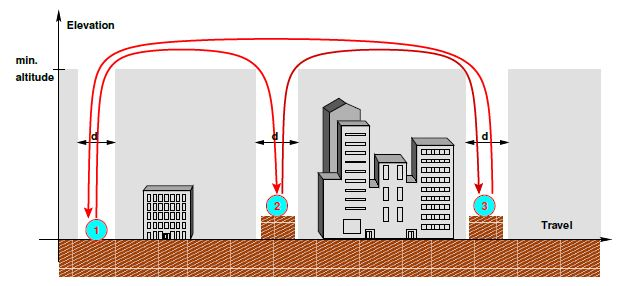
\includegraphics[scale=0.7]{hauptaufgabe} 
		\caption{Flugbahn der Hauptaufgabe}
		\label{fig:hauptaufgabe}
	\end{center}
	
	\begin{center} 
		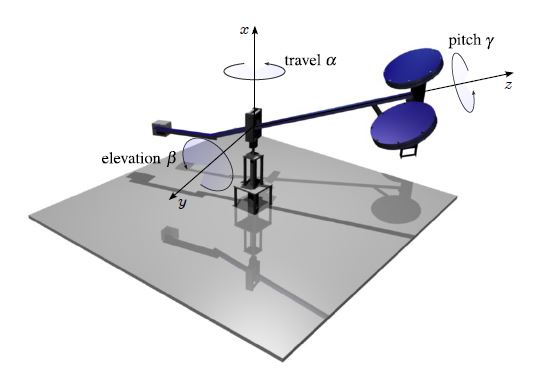
\includegraphics[scale=0.7]{koordinatensystem} 
		\caption{Darstellung des Versuchsaufbaus}
		\label{fig:koordinatensystem}
	\end{center}
\end{figure}

\section{Modellierung}


\section{Referenztrajektorie}
Um die Aufgabe zu absolvieren, ist es notwendig, die Referenzsignale zu definieren. Diese Signale muss die vorgegebene Anforderungen erfüllen. Die Hauptaufgabe lassen sich wie Tabelle 1 definieren.
\begin{table}[H]
	\caption{Hauptaufgabe}
	\centering
	%\textcolor{red}{Tabelle mit Werten füllen + vervollständigen}
	%\label{table:parameters}	
	\begin{tabular}{|c|c|c|c|}
		\hline
		\bfseries Subtask & \bfseries Point & \bfseries $\alpha$ & \bfseries $\beta$ \\ \hline \hline
		Start	& $1$ & 0\degree & approx. -27\degree\\ \hline
		Cargo pick-up	& $2$ & 90\degree  &  approx. -22\degree  \\ \hline
		Cargo deposition & $3$ & 450\degree&  approx. -22\degree  \\ \hline
		Finish(landing) & $1$ & 0\degree &  approx. -27\degree  	\\ \hline
	\end{tabular}
\end{table}

Außerdem ist die Mindestflughöhe von Steigwinkel $\beta$ gleich $-7.5\degree$. Weil der Nickwinkel $\gamma$ nicht berücksichtigt wird, ist es nur notwendig, Referenzsignale für Schwenkwinkel $\alpha$ und Steigwinkel $\beta$ zu definieren. Die Trajektorie soll in einige Abschnitte unterteilt werden, in denen jeweils ein Zustand verändert wird. Es gibt verschiedene Möglichkeiten, wie z.B. Sprünge, Rampen, trigonometrische Funktionen(wie $\sin$ und $\cos$) oder Polynome n-ten Grades, um die Zustandsänderung bei jedem Abschnitt darzustellen. Hier wurden Sinus-Funktionen mit verschiedenen Zeitpunkten implementiert. Durch Phasenverschiebung ($\pi/2$) können die steigenden Sinus-Signale und die fallenden Sinus-Signale unterscheidet werden. Die steigenden Signale werden durch
\begin{equation}
    S_{steig}=Z \pm Zsin(\frac{2\pi(t-T_{start})}{2(T_{end}-T_{start})}-\pi/2)
\end{equation}
gegeben. Die fallende Signale werden durch
\begin{equation}
	S_{fall}=Z \pm Zsin(\frac{2\pi(t-T_{start})}{2(T_{end}-T_{start})}+\pi/2)
\end{equation}  
gegeben. Z ist die Amplitude bei jeder Abschnitt. $T_{start}$ ist der Startzeitpunkt von jedem Abschnitt. $T_{end}$ ist der Endzeitpunkt. Die Abschnitte lassen sich wie in Tabelle 2 definieren.
\begin{table}[H]
	\caption{Trajektorieabschnitte}
	\centering
	%\textcolor{red}{Tabelle mit Werten füllen + vervollständigen}
	%\label{table:parameters}	
	\begin{tabular}{|c|c|c|c|}
		\hline
		\bfseries Abschnitt & \bfseries $\alpha$ & \bfseries $\beta$ & \bfseries Aufgabe \\ \hline \hline
		1 & 0\degree & -27\degree & Start \\ \hline
		2 & 0\degree & -27\degree$\rightarrow$0\degree & /  \\ \hline
		3 & 0\degree & 0\degree & / \\ \hline
		4 & 0\degree$\rightarrow$90\degree & 0\degree  & / 	\\ \hline
		5 & 90\degree & 0\degree & /  	\\ \hline
		6 & 90\degree & 0\degree$\rightarrow$-22\degree & /  \\ \hline
		7 & 90\degree & -22\degree & Cargo Pick-up  	\\ \hline
		8 & 90\degree & -22\degree$\rightarrow$0\degree & /  \\ \hline
		9 & 90\degree & 0\degree & /  	\\ \hline
		10 & 90\degree$\rightarrow$450\degree & 0\degree & /  	\\ \hline
		11 & 450\degree & 0\degree & / 	\\ \hline
		12 & 450\degree & 0\degree$\rightarrow$-22\degree & /  	\\ \hline
		13 & 450\degree & -22\degree & Cargo deposition  	\\ \hline
		14 & 450\degree & -22\degree$\rightarrow$0\degree & /  	\\ \hline
		15 & 450\degree & 0\degree & /  	\\ \hline
		16 & 450\degree$\rightarrow$0\degree & 0\degree & /  	\\ \hline
		17 & 0\degree & 0\degree & /  	\\ \hline
		18 & 0\degree & 0\degree$\rightarrow$-27\degree & /  	\\ \hline
		19 & 0\degree & -27\degree & Finish(landing)  	\\ \hline
	\end{tabular}
\end{table}
 
Fig. 3 und 4 zeigen die Solltrajektorie in $\alpha$ und $\beta$ Richtung.


\begin{figure}[ht]
	\begin{center} 
		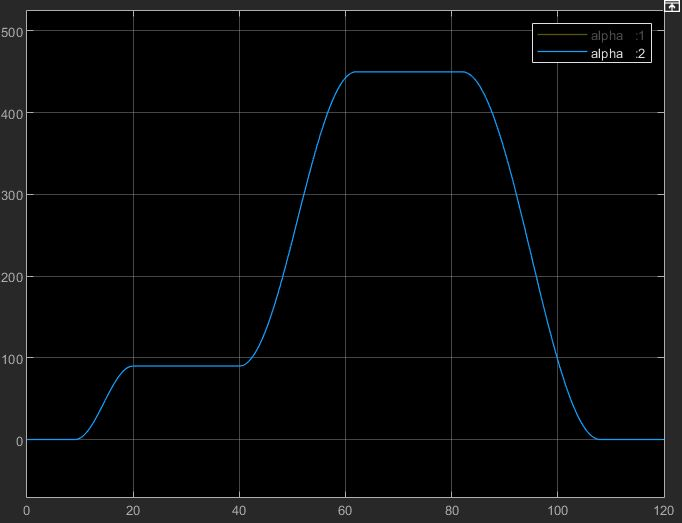
\includegraphics[scale=0.55]{alphasoll} 
		\caption{Sollsignal von $\alpha$}
		\label{fig:alphasoll}
	\end{center}
	
	\begin{center} 
		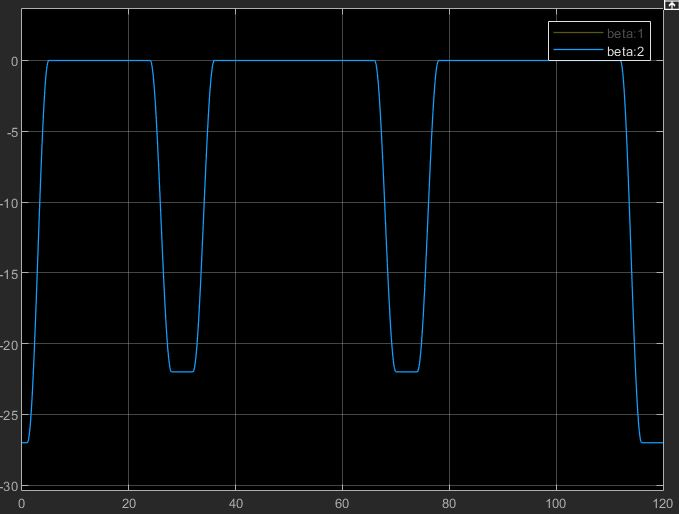
\includegraphics[scale=0.55]{betasoll} 
		\caption{Sollsignal von $\beta$}
		\label{fig:betasoll}
	\end{center}
\end{figure}

\section{LQI-Regler}


\section{Simulationsergebnisse}

Nach dem Entwurf des Reglers wird das komplette System mit dem Black Box Modell getestet. Bei dem Black Box Modell muss man die Vorzeichen von $\alpha$, $\beta$, und $\gamma$ beachten. Wenn die Vorzeichen falsch sind, funktioniert der Regler schlecht. Die Solltrajektorie wird in das System eingegeben, um die Funktion des Regler zu prüfen. Nach Auswahl passender Parameter kann die Gesamtaufgabe unter 120s gelöst werden. In Fig.5 und 6 sind die Verläufe des Schwenkwinkelsignals($\alpha$) und des Steigwinkelsignals($\beta$). Der Signalverlauf der Solltrajektorie sind in den Abbildungen mit blau gekennzeichnet, während die geregelte Strecke in gelb gekennzeichnet ist. Aus den Abbildungen sieht man deutlich, dass das Verhalten des Reglers ausgezeichnet ist.

\begin{figure}[ht]
\begin{center} 
	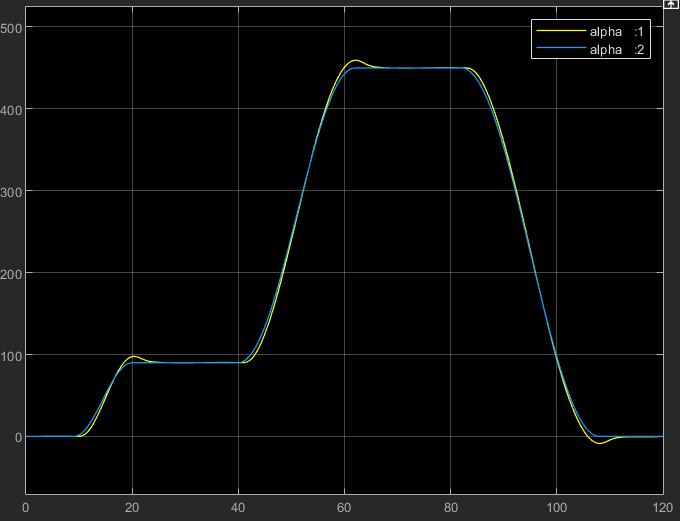
\includegraphics[scale=0.55]{alpha_final} 
	\caption{Ergebnis des Black Box Modells in $\alpha$}
	\label{fig:alpha_bbm}
\end{center}

\begin{center} 
	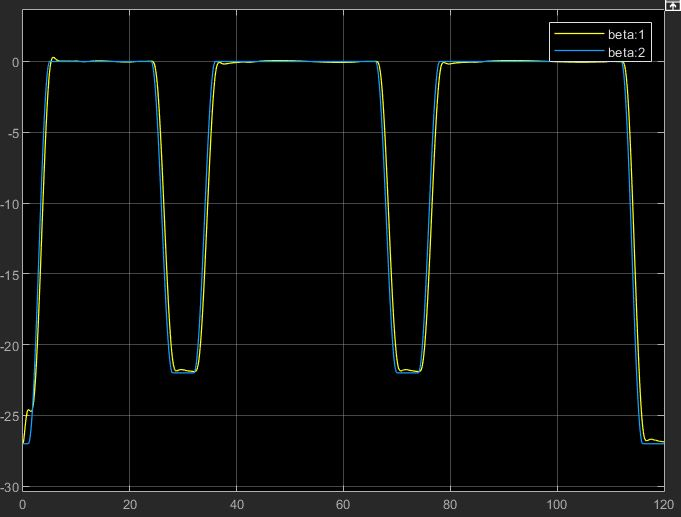
\includegraphics[scale=0.55]{beta_final} 
	\caption{Ergebnis des Black Box Modells in $\beta$}
	\label{fig:beta_bbm}
\end{center}

\end{figure}

\section{Fazit}
In diesem Protokoll stellen wir unsere Arbeit für das Praktikum Konzept der Regelungstechnik vor, in der wir einen beobachterbasierten LQI-Regler für den 3-DOF Helikopter entworfen haben.  Wir verwendeten den systematischen Ansatz zur Lösung allgemeiner Regelungsprobleme. Wichtige Schritte in diesem Prozess waren die Modellierung des Systems, die Wahl der Regelstruktur und des eigentlichen Reglertyps und schließlich die Implementierung und Validierung des entworfenen Reglers. Außerdem ist eine ordentliche Dokumentationen von Ergebnissen auch wichtig, da diese eine Richtlinie sind. Die Betreuung der Tutoren während des Praktikums ist sehr hilfreich. Zusammenfassend lässt sich sagen, dass wir viele praktische Erfahrungen gesammelt haben und diese Erfahrungen auf weitere Aspekte im Studium sowie im Berufsleben anwenden können.
%\bibliographystyle{alpha}        % Include this if you use bibtex 
%\bibliography{autosam}           % and a bib file to produce the 
%\bibliography{autosam}
                                 % bibliography (preferred). The
                                 % correct style is generated by
                                 % Elsevier at the time of printing.

\begin{thebibliography}{1}
	
\bibitem{handbook}Handbook Control of a 3-DOF Helicopter
\\ IST, University of Stuttgart, Germany
\\ Corona Edition Winter term 2020/21
	
\bibitem{Regelkreisstrukturen}Regelkreisstrukturen
\\ IST, University of Stuttgart, Germany	

	
	
	
\end{thebibliography}

%\appendix
\end{document}